\documentclass[12pt]{article}
\usepackage{fullpage}
\usepackage{graphicx, rotating, booktabs} 
\usepackage{times} 
\usepackage{fbb} 
\usepackage{natbib} 
\usepackage{indentfirst} 
\usepackage{setspace}
\usepackage{grffile} 
\usepackage{hyperref}
\usepackage{tikz-cd}
 \usetikzlibrary{cd}
\usepackage[export]{adjustbox}
\usepackage[most]{tcolorbox}
\usepackage{verbatimbox}
\usepackage{lscape}
\usepackage{afterpage}
\usepackage{amsmath}
\usepackage[labelfont={bf},textfont=it,labelsep=period]{caption}
 \usepackage{multirow} 
\setcitestyle{aysep{}}
\usepackage{dcolumn}

\hypersetup{
  colorlinks = true,
  urlcolor = blue,
  linkcolor = black,
  citecolor = black,
  pdfauthor = {Joshua Alley},
  pdfkeywords = {},
  pdftitle = {},
  pdfsubject = {},
  pdfpagemode = UseNone,
%  pdffitwindow = true
%  pdfcenterwindow = true
}



\singlespace
\title{\textbf{Using Hierarchical Models to Estimate Heterogeneous Effects}}
\author{Joshua Alley \\
Assistant Professor \\
University College Dublin \\
joshua.alley@ucd.ie
}

 
\date{\today}

\bibliographystyle{apsr}

\usepackage{sectsty}
\sectionfont{\Large}
\subsectionfont{\noindent\large\textit}
\subsubsectionfont{\normalsize}

\makeatletter
\renewcommand\tiny{\@setfontsize\tiny{9}{10}}
\makeatother


\begin{document}

\maketitle 

\begin{abstract} 
%Heterogeneous effects are common in social science. 
This note describes how and when to use Bayesian hierarchical models to estimate heterogeneous effects. 
While an ample literature suggests that hierarchical models provide helpful regularization and information about variation, political scientists rarely use them to estimate heterogeneous effects. 
Doing so is simple, however. 
To start, specify groups based on quantities of interest such as demographics, context, and policy relevance.  
Then, fit a hierarchical model where treatment slopes and intercepts vary across groups.
This captures systematic and random variation in heterogeneous effects, estimates effects within each group, and measures effect variance. 
Hierarchical modeling provides an intermediate tool between interactions or subgroup analyses and machine learning approaches to discovering complex heterogeneity. 
It is more flexible than interactions and reduces the risk of underpowered subgroup comparisons.
At the same time, it is more theoretically informed and interpretable than some machine learning approaches, as well as easier to implement in small datasets. 
Researchers can thus use hierarchical models alongside other approaches to understand heterogeneous effects for scholarship and policy.
\end{abstract} 


\newpage 
\doublespace 


\section{Introduction}


% one: het effects matter
Whether in observational or experimental studies, every independent variable social scientists examine impacts some units differently than others. 
Common estimands aggregate heterogeneous effects.\footnote{For instance, \citet{Abramsonetal2022} note that the average marginal component effect (AMCE) of conjoint experiments gives more weight to intense preferences.} 
These average effects are useful, but they often obscure interesting and important variation. 


As a result, understanding heterogeneous effects is essential for policy and scholarship. 
Estimating heterogeneity allows scholars to clarify the connection between their independent variable and outcome.
Policymakers can maximize the impact of finite resources with targeted interventions, for example by providing job training to individuals who are more likely to benefit. 
% expand/sharpen this, if there is space. (There is not for PA) 


% two: introduce my solution 
This letter explains how and when to use hierarchical models to estimate heterogeneous effects. 
I identify when researchers can profitably use hierarchical models, and when other tools make more sense. 
A large statistics literature suggests that Bayesian hierarchical models are a useful tool for  heterogeneous effects estimation (e.g., \cite{FellerGelman2015, McElreath2016, Dorieetal2022}).
Political scientists tend to rely on interactions or machine learning tools instead, however.  
For instance, of the three applied political science citations of \citet{FellerGelman2015}, only \citet{Marquardt2022} models treatment effects. 


% three: loads of techniques
Hierarchical modeling of heterogeneous effects fills a gap between interactions and machine learning.\footnote{\citet{BlackwellOlson2022} describe a lasso approach to interactions that sits between machine learning and linear regressions.}
Parametric interactions and subgroup analyses are ubiquitous because they are easy to interpret.
These approaches are hard to interpret with more than three dimensions and are often underpowered \citep{Simmonsetal2011}.
More recent work employs random forests \citep{GreenKern2012, WagerAthey2018}, support vector machines \citep{ImaiRatkovic2013}, and ensemble methods \citep{Grimmeretal2017, Kuenzeletal2019, Dorieetal2022}.
These machine learning algorithms can discover complex patterns and high-dimensional variation, but can be difficult to interpret and implement, especially in smaller social science datasets.

 
Using a hierarchical model is more flexible than parametric interactions but easier to implement and interpret than machine learning approaches.  
It preserves a simple and interpretable structure, while accommodating more factors and ameliorating the downsides of subgroup analysis via partial pooling. 
This facilitates argument testing.
Unlike machine learning, the hierarchical approach lacks the flexibility to discover high-dimensional heterogeneity, however.  



Hierarchical modeling therefore works best when there are more than two modifying factors and therefore many subgroups of interest, as well as less emphasis on discovery. 
These models are best at capturing variation across groups and levels when there are multiple potential modifiers.
Considering multiple modifiers is important because social scientists often posit conditional theories with a single modifier. % may need to expand or find a new home 


There are two key steps when theory and data make using hierarchical models worthwhile.
First, researchers should define groups based on potential sources of heterogeneity such as other treatments, context, demographics, or policy concerns. 
Second, they should estimate heterogeneous effects across those groups using a hierarchical model with varying slopes and intercepts, along with covariates that predict slopes.
Modeling heterogeneous effects in this way produces interpretable results, which facilitates argument testing.
It also allows researchers to examine effects within groups, compare different sources of heterogeneous effects and describe how much an effect varies.  


While frequentist estimation of hierarchical models is possible, Bayesian estimation is straightforward and more informative.
Bayesian estimation provides crucial information by connecting parameters through common prior distributions, thereby regularizing estimates and propagating uncertainty. 
Working with posterior distributions also gives researchers more flexibility to present diverse information about how and when effects vary. 
While computation and coding were once a barrier to employing Bayesian methods, fitting a wide range of hierarchical models is straightforward with the brms package in \textsf{R} \citep{Buerkner2017}.\footnote{I provide example code in this note and the appendix.}
Calculating substantive effects is also simple \citep{ArelBundockme}.



% wrap and introduce the application 
In the remainder of this note, I describe how and when to estimate hierarchical models of heterogeneous effects and demonstrate the process by analyzing a study of how military alliances shape public support for war by \citet{TomzWeeks2021}. 
The reanalysis reveals that alliances increase support for intervention most among white men who support international engagement but are otherwise skeptical of using force. 
%Alliances increase mass support for war by impacting individuals who otherwise prefer peaceful collaboration. 



\section{Hierarchical Modeling of Heterogeneous Effects}


There are two steps in hierarchical models of heterogeneous effects. 
First, researchers must define the groups over which an independent variable's impact changes. 
Unique combinations of characteristics such as other treatments, context and demographics determine groups.


Researchers should create groups based on what variation is most important and interesting. 
Theory, policy concerns, or normative factors are all possible motivations. 


Setting groups is the most important task, because it determines what heterogeneous effects a researcher estimates. 
Defining groups before model fitting defines what variation is most important, links heterogeneous effects to theory, and structures modeling.\footnote{It also facilitates pre-registration when applicable.}
Defining groups without careful thought risks obfuscating results and can hinder model fitting.   


% three ways to set groups
There are three general approaches to defining groups.  
First, researchers can set groups using combinations of other treatments, especially when an intervention has several dimensions but theory emphasizes one of them. 
The experimental design determines groups, and the model estimates heterogeneous treatment effects.   
If researchers want to know how different issues shape the impact of elite foreign policy cues \citep{GuisingerSaunders2017}, they could define groups by issues, for instance.
Hierarchical estimators for topic-sampling experiments apply this idea to estimate how a treatment varies across different topics \citep{CliffordRainey2023}. 
Researchers sometime use fully crossed interactions to estimate the impact of a treatment across experimental strata. 


A second approach uses unit, demographic and contextual factors to create groups and estimate  effect heterogeneity. 
Here, researchers examine what factors within or around units shape their response to an independent variable.
For example, \citet{Alley2021isq} uses alliance characteristics to examine when alliance membership increases or decreases military spending.
Other use cases include estimating how different demographic groups or geographic units respond to an intervention.
One might examine how the impact of a national-level intervention varied across states, for example.\footnote{Extrapolation to a representative sample for such units might require poststratification.}


Third, researchers might use hierarchical models to address specific policy concerns.
Policy analysts often want to know how an intervention impacts a specific population. 
Researchers might want to know if a job-training program improves employment outcomes for black women in the South, for instance.  


% grouping factors: numbers 
Whether researchers use other treatments, context, or policy to determine groups, the number of grouping factors depends first on theory.
There are some practical constraints, however.
Using too many factors can lead to model fitting and interpretation problems by creating many small groups.
How many factors is too many depends especially on the data- some datasets can support reasonably large groups for many factors. 
At the other extreme, using only one grouping factor will add relatively little value compared to interactions. 



After defining groups, the second step is fitting a hierarchical model of effects within groups.
The model employs a mix of varying intercepts and slopes to estimate the impact of an intervention in each group.\footnote{If other units such as states define the groups, rather than combinations of modifying variables, then adding group-level predictors is essential. For examine, in a model where an effect varies by state, adding state-level variables like ideology, population and GDP would avoid partially pooling small groups too far towards the overall mean.}
%The first equation links the independent variable and outcome.
%The second equation estimates heterogeneous effects as a function of group characteristics.
%The second equation is essential, as group variables add substantial information and avoid simply pooling small groups towards the overall mean.
%Without the group predictors, the random effects of each treatment will shift towards the mean because the information about each group depends only on how many data points it contains. 


This approach can address diverse problems, but for ease of exposition consider making between-unit comparisons based on an experimental treatment.    
Start with \textit{N} units indexed by \textit{i}, some of which receive a binary treatment \textit{T}.
Assume that the outcome variable ${y}$ is normally distributed with mean $\mu_i$ and standard deviation $\sigma$.\footnote{Researchers should use binary, categorical and other outcome likelihoods.}
\textit{g} indexes the researcher-defined groups, which include two variables \textit{v1} and \textit{v2}. 


%The first equation predicts the outcome mean. 
The outcome for each unit is then a function of group varying intercepts $\alpha_g$, an optional matrix of control variables \textbf{X}, and a set of group treatment effects $\theta_g$, which are normally distributed with mean $\eta_g$ and standard deviation $\sigma_\theta$. 
The researcher divides all units into \textit{g} groups based on unique combinations of heterogeneous effect predictors \textbf{Z}. 
Each $\theta$ parameter estimates how the treatment effect varies across the values of  each variable.  
To capture correlations between the random intercepts and varying slopes $\rho \sigma_\alpha \sigma_\theta$, these variables should have a common multivariate normal prior.


\begin{align*}
y_i &\sim N(\mu_i, \sigma) &\text{(Likelihood)} \\
\mu_i &= \alpha + \alpha_{v1} + \theta_{v1} + \textit{T} + \alpha_{v2} + \theta_{v2} \textit{T} + \textbf{X} \beta &\text{(Outcome Equation)}  \\ 
\begin{pmatrix} 
\alpha_{v1} \\
\theta_{v1} \\
\end{pmatrix} &\sim  N
\begin{bmatrix}
\begin{pmatrix}
\mu^\alpha_{v1} \\
\mu^\theta_{v1} \\
\end{pmatrix}\!\!,&
\begin{pmatrix}
\sigma^2_\alpha & \rho \sigma^\alpha_{v1} \sigma^\theta_{v1} \\
\rho \sigma^\alpha_{v1} \sigma^\theta_{v1} & \sigma^2_\theta \\
\end{pmatrix}
\end{bmatrix} & \text{(Correlated Intercepts and Slopes: V1)} \\ 
\begin{pmatrix} 
\alpha_{v2} \\
\theta_{v2} \\
\end{pmatrix} &\sim  N
\begin{bmatrix}
\begin{pmatrix}
\mu^\alpha_{v2} \\
\mu^\theta_{v2} \\
\end{pmatrix}\!\!,&
\begin{pmatrix}
\sigma^2_\alpha & \rho \sigma^\alpha_{v2} \sigma^\theta_{v2} \\
\rho \sigma^\alpha_{v2} \sigma^\theta_{v2} & \sigma^2_\theta \\
\end{pmatrix}
\end{bmatrix} & \text{(Correlated Intercepts and Slopes: V2)} \\ 
\theta_g &= \theta_{v1} \textit{V1} + \theta_{v2} \textit{V2} & \text{(Group Slopes)} \\
\alpha_g &= \alpha_{v1} + \alpha_{v2} & \text{(Group Intercepts)} \\
%\mu_\theta &= \lambda_0 + \textbf{Z} \lambda &\text{(Heterogeneous Effects)} 
\end{align*}


This approach lets slopes vary across multiple variables within a group. 
The net impact of the treatment in each group depends on the linear combination of slopes in that group, specifically the $\theta$ parameters and values of each variable. 
Similarly, the group intercepts can be calculated as the sum of the corresponding random intercepts for each grouping variable.\footnote{In brms for a model with no controls and two variables modifying the impact of a treatment, the model formula is y $\sim$ 1 + (1 + treat | var1) + (1 + treat | var2). If joint variation across variables 1 and 2 is also of interest, append (1 + treat | var1:var2).}  


%The heterogeneous effects equation then predicts the treatment effects with the matrix \textbf{Z}, which contains unique combinations of whatever variables define the groups.  
%As a result, each $\theta$ reflects a unique mix of factors that modify the treatment.
%The second equation also includes an intercept $\lambda_0$ that estimates the impact of treatment when all sources of heterogeneity are zero.\footnote{In brms for a model with no controls and two variables modifying the impact of a treatment, the model formula is y $\sim$ 1 + treat*(var1 + var2) + (1 + treat | var1:var2). treat*(var1 + var2) expresses part of the second equation, while (1 + treat | var1:var2) lets slopes vary by group.}


The above model can be fit with Bayesian or frequentist methods, but Bayesian estimation offers some useful advantages.
First, it is more flexible, and including prior information can facilitate model fitting and convergence. 
Priors also help regularize estimates by pulling extreme groups towards the overall mean.
Working with posterior distributions also also provides a wealth of information about effect heterogeneity and propagates uncertainty.  


% Interpretation 
In interpreting these models, researchers should leverage the full range of information from the different parameters. 
First, the $\theta$ posteriors give the impact of a variable within each group.
All $\theta$s reflect a systematic component from the predictors in \textbf{Z}$\lambda$ and a random variation in slopes from $\sigma_\theta$. 
Unless the group-level predictors are weak correlates of treatment response, the systematic component will dominate. 
The random variation is similar to the error term in regression- it expresses how much variation is left in addition to the systematic component. 


% additional information 
In addition to group-specific effect estimates, a hierarchical model facilitates rich description of effects across groups. 
It estimates how specific factors drive differences between groups via the $\lambda$ parameters.
Researchers can also calculate variance in the $\theta$ parameters across groups and compare the posteriors of different $\theta$s. 
The $\sigma_\theta$ parameter summarizes the random variation. 
Other techniques such as interactions in OLS with robust standard errors provide less information.


\section{When to Use Hierarchical Models}

% advantages 
In deciding whether to use hierarchical models, researchers must weigh it's unique advantages and disadvantages. 
In general, estimating heterogeneous effects in this way has three advantages.
First, researchers can make detailed inferences about heterogeneous effects in an interpretable framework. 
This helps examine theories that predict how an effect varies and compare sources of variation.\footnote{Rescaling variables in the heterogeneous effects equation can aid model fitting and coefficient comparisons \citep{Gelman2008}.} 
Partial pooling also facilitates reasonable estimates for small groups by sharing information across groups and incorporating predictors in the heterogeneous effects equation. 
Finally, this approach will be faster than machine learning approaches for many datasets, easier to use in small datasets, and may scale better than models of individual treatment effects.


% disadvantages
Like all methods, the hierarchical approach has downsides, some of which can be ameliorated with modifications, while others should lead researchers to use different tools. 
Because groups are based on unique combinations of heterogeneous effect variables, using multiple continuous variables in the heterogeneous effects equation creates many small groups or individual treatment effects, which increases the risk of sampling problems, especially in small datasets. 
If using continuous variables hinders model convergence, researchers can bin continuous variables.


Furthermore, hierarchical models can show general trends, but will not make powerful comparisons between every group. 
Researchers who want to compare specific groups may lack empirical leverage, especially for small groups.


% Relative to interactions
With these considerations in mind, when should researchers use hierarchical models in place of interactions?
If only one factor modifies an effect, interactions are best, as the extra information hierarchical models provide is less valuable. 


% two modifiers
With two or more modifiers, hierarchical models begin to add value beyond interactions. 
Interpreting triple interactions between a variable and two modifiers is challenging. 
The advantages of hierarchical modeling increase with the number of modifiers, until additional modifiers create small groups that complicate model fitting. 
The thresholds where the number of modifiers becomes an issue for hierarchical modeling depends on the data, as larger datasets can support more groups. 


% not as well suited for discovery 
The relative use cases of hierarchical models and machine learning are different. 
Unlike machine learning approaches, hierarchical models will not discover high-dimensional interactions. 
Researchers can add flexibility with additional interactions or non-linear specifications in either level of the model, but this requires a priori specification. 
Therefore, if researchers want to focus on flexible discovery, not testing an argument with multiple sources of treatment heterogeneity, they should rely more on machine-learning. 


In summary, researchers should continue to use interactions for single modifiers and machine learning to discover complex interactions. 
Hierarchical modeling works well when there are two or more modifiers and researchers have adequate data to support an informative model.  
\autoref{tab:tools-det} summarizes some relevant characteristics of hierarchical, interaction and machine learning approaches to heterogeneous effects. 
Hierarchical modeling is thus an intermediate tool between interactions and machine-learning, where researchers need more flexibility than interactions but are not willing or able to tackle the computational and interpretation challenges of machine learning. 


\begin{table}
\begin{tabular}{|p{1in}|p{1.5in}|p{1.5in}|p{1.5in}|} \hline
                 & Hierarchical Models & Interactions/Subgroup & Machine Learning \\
\hline
Factors              & Two or more          & One or two         & Many \\ \hline
Sample Size          & Conditional on number of factors            & Medium to large, depending on main effect size    & Large \\ \hline
Complexity           & Medium             & Low                & High \\ \hline
Computational Cost   & Medium             & Low                & High \\ \hline
Interpretability     & High               & High               & Low \\ \hline
Modifiers            & Specified          & Specified      & Discovered or Specified \\
\hline
\end{tabular}
\caption{Key characteristics of different approaches to estimating heterogeneous effects.}
\label{tab:tools-det}
\end{table}


\section{Example Application} 


In the following, I demonstrate how the hierarchical approach works by reanalyzing a study by \citet{TomzWeeks2021} (TW hereafter). 
TW examine whether the public is more willing to go to war for an allied country.
In a factorial experiment with vignettes, they find a 33\% average increase in support for military intervention on behalf of another country if that country is an ally. 
This is a large and potentially important effect, so I estimate who responds to alliances.\footnote{See the appendix for a heterogeneous treatments analysis that corroborates TW's results.}


I used race, gender, hawkishness and internationalism to define demographic groups and predict treatment heterogeneity across those groups. 
I selected these variables because foreign policy dispositions like militant assertiveness shape general willingness to use force \citep{Kertzeretal2014} as do gender \citep{Barnhartetal2020} and race. 
I also control for other experimental manipulations.\footnote{See the appendix for priors.} 
Following TW's OLS analysis, I use a Gaussian likelihood, although the outcome is a binary variable. 


I describe the results in two steps. 
First, I summarize the predictors of the alliance effect in \autoref{fig:tw-het-source}.
I then present the resulting heterogeneous effects for every group in \autoref{fig:tw-treat-het}.


\begin{figure}[htpb]
	\centering
		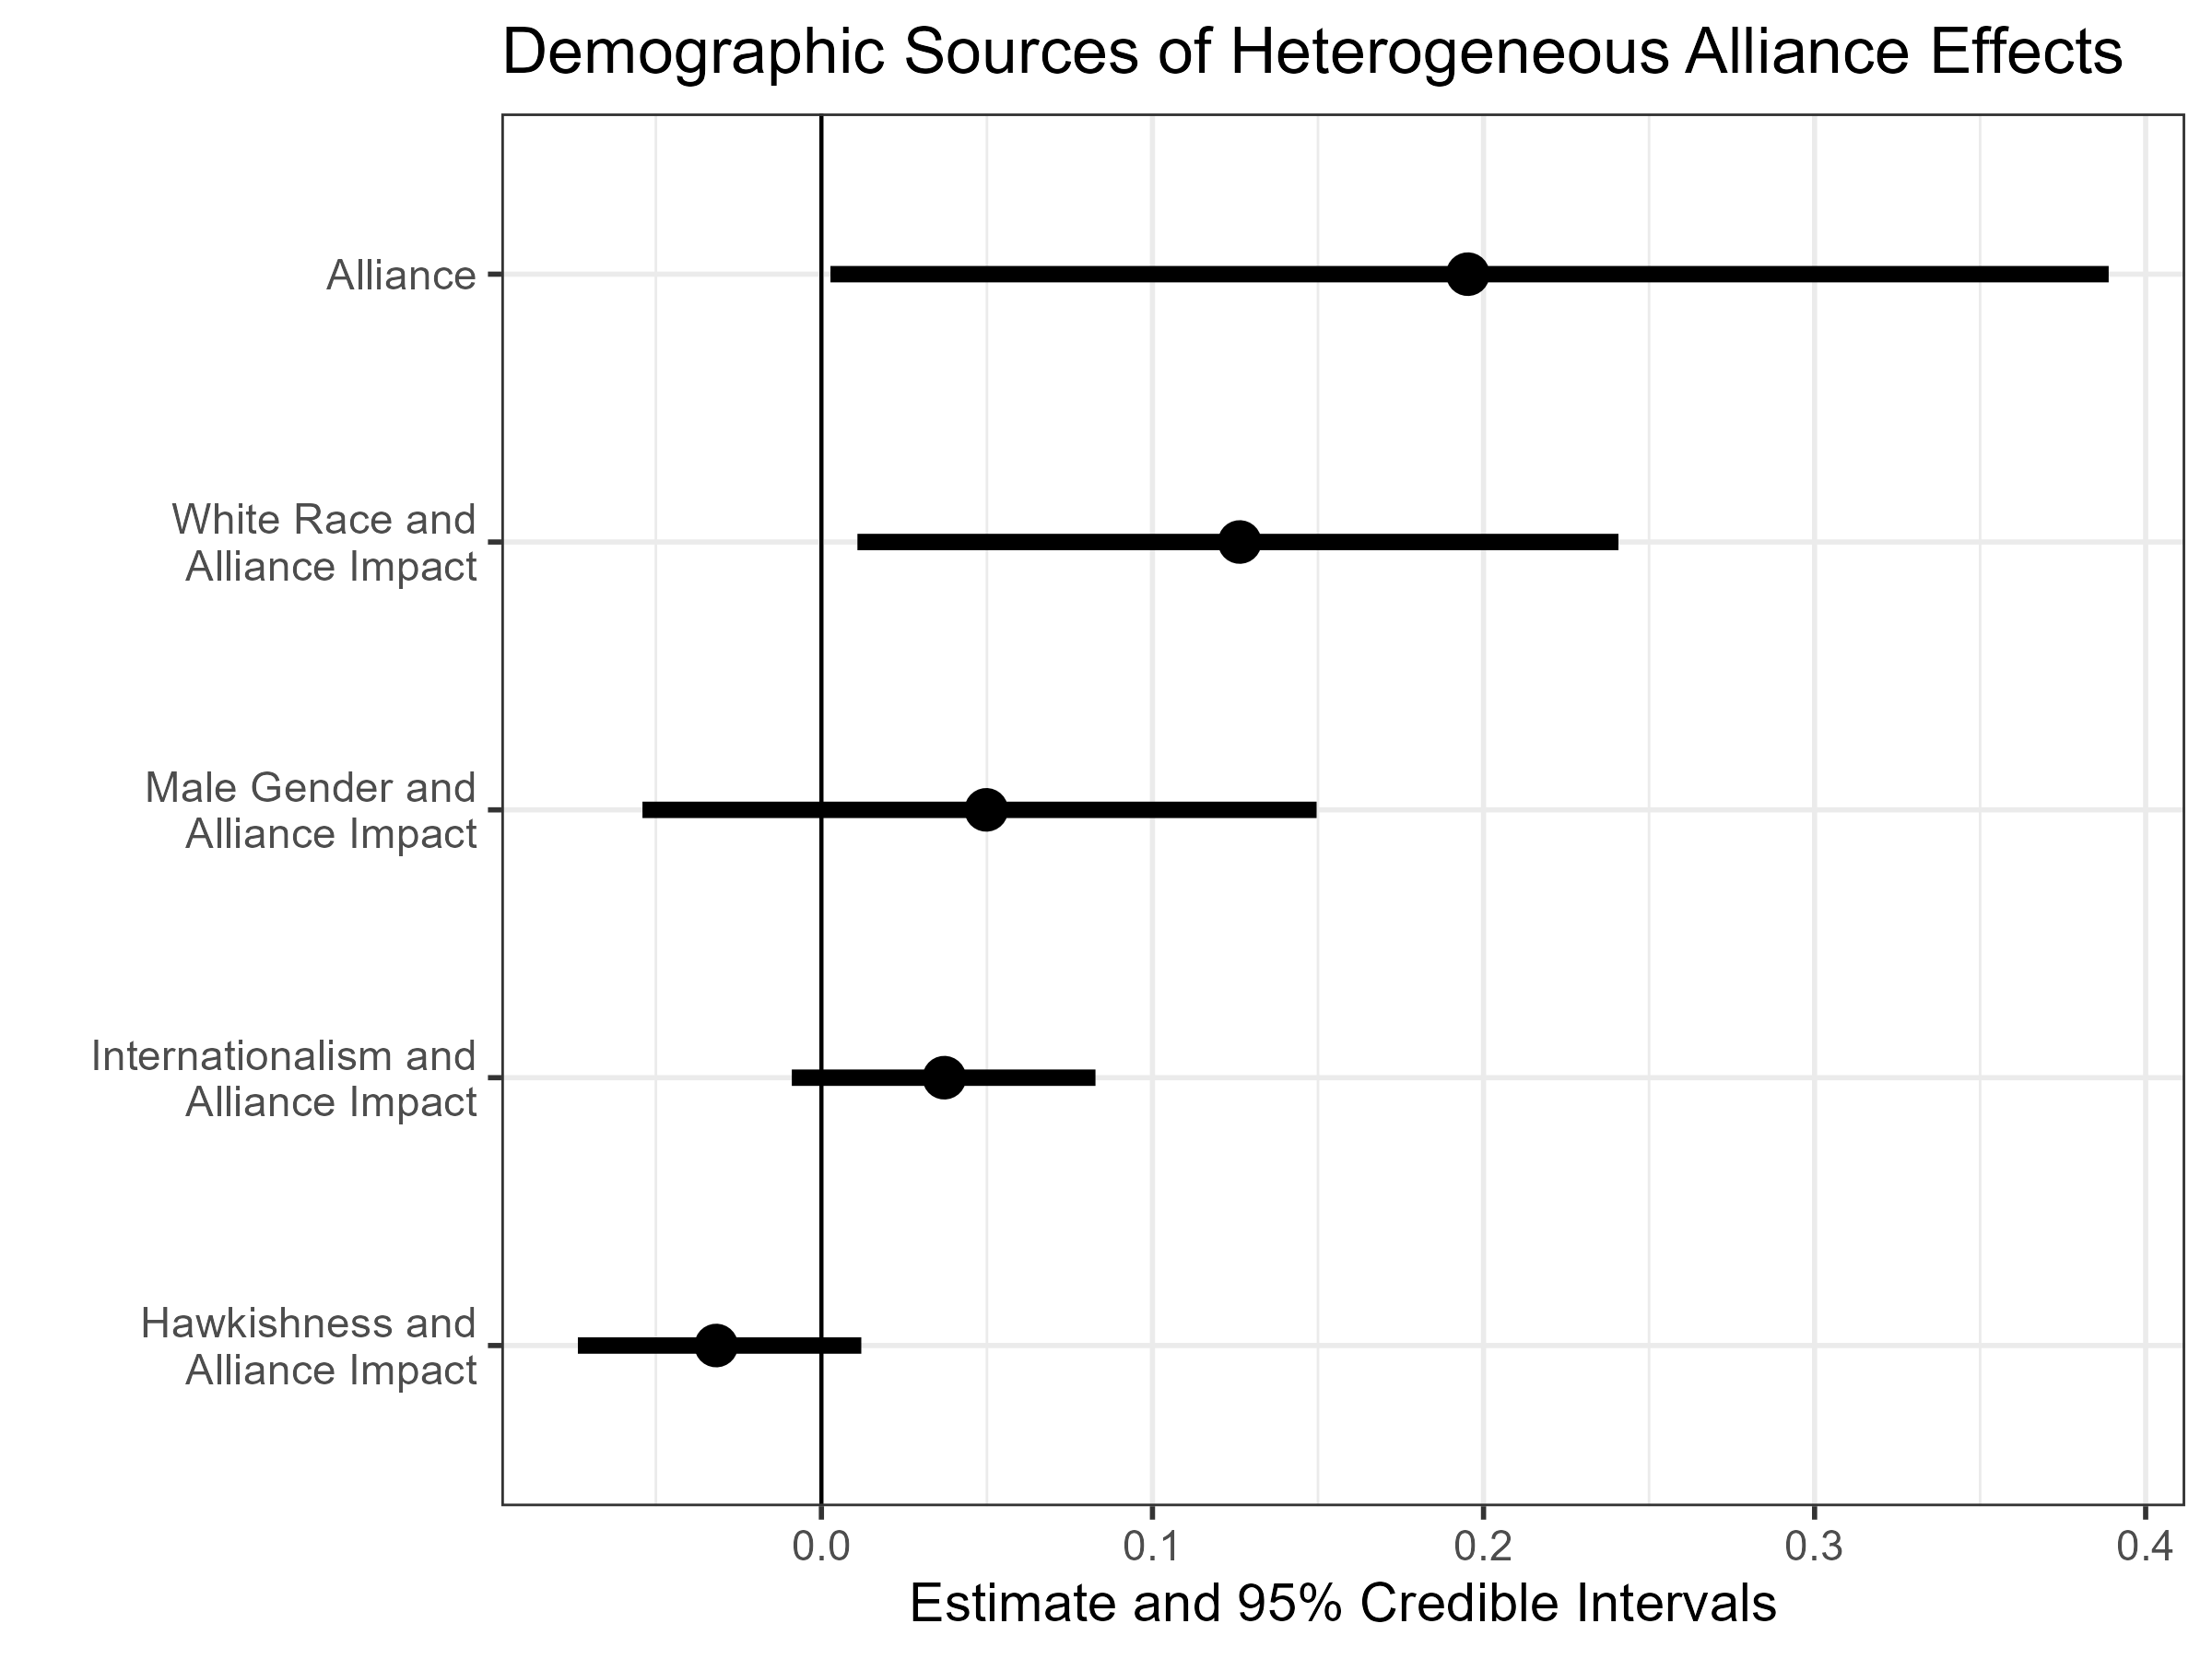
\includegraphics[width=0.95\textwidth]{../figures/tw-het-source.png}
	\caption{Heterogeneous effects equation coefficients from a hierarchical model of how military alliances impact public support for war. Hawkishness, internationalism, white race and male gender predict the impact of alliances.}
	\label{fig:tw-het-source}
\end{figure}


\autoref{fig:tw-het-source} plots how support for international engagement, willingness to use force, race and gender modify the impact of alliances.\footnote{These are the $\lambda$ parameters above.}
These group-level predictors modify the treatment effect.
Each coefficient therefore expresses whether a variable increases, decreases, or has no relationship with the impact of alliances on support for military intervention.  


The top coefficient estimate, ``Alliance'' indicates that when all group variables are 0, alliances increase support for intervention by 20\%. 
The white race coefficient suggests that alliances increase support for intervention by 12\% more among white respondents than non-white respondents. 
Next, men are marginally more responsive to alliances than women, but this difference has positive, negative and zero values.  
As internationalism increases, the impact of alliances rises by 4\% in expectation.
Conversely, greater hawkishness marginally attenuates the impact of an alliance. 


\begin{figure}[htpb]
	\centering
		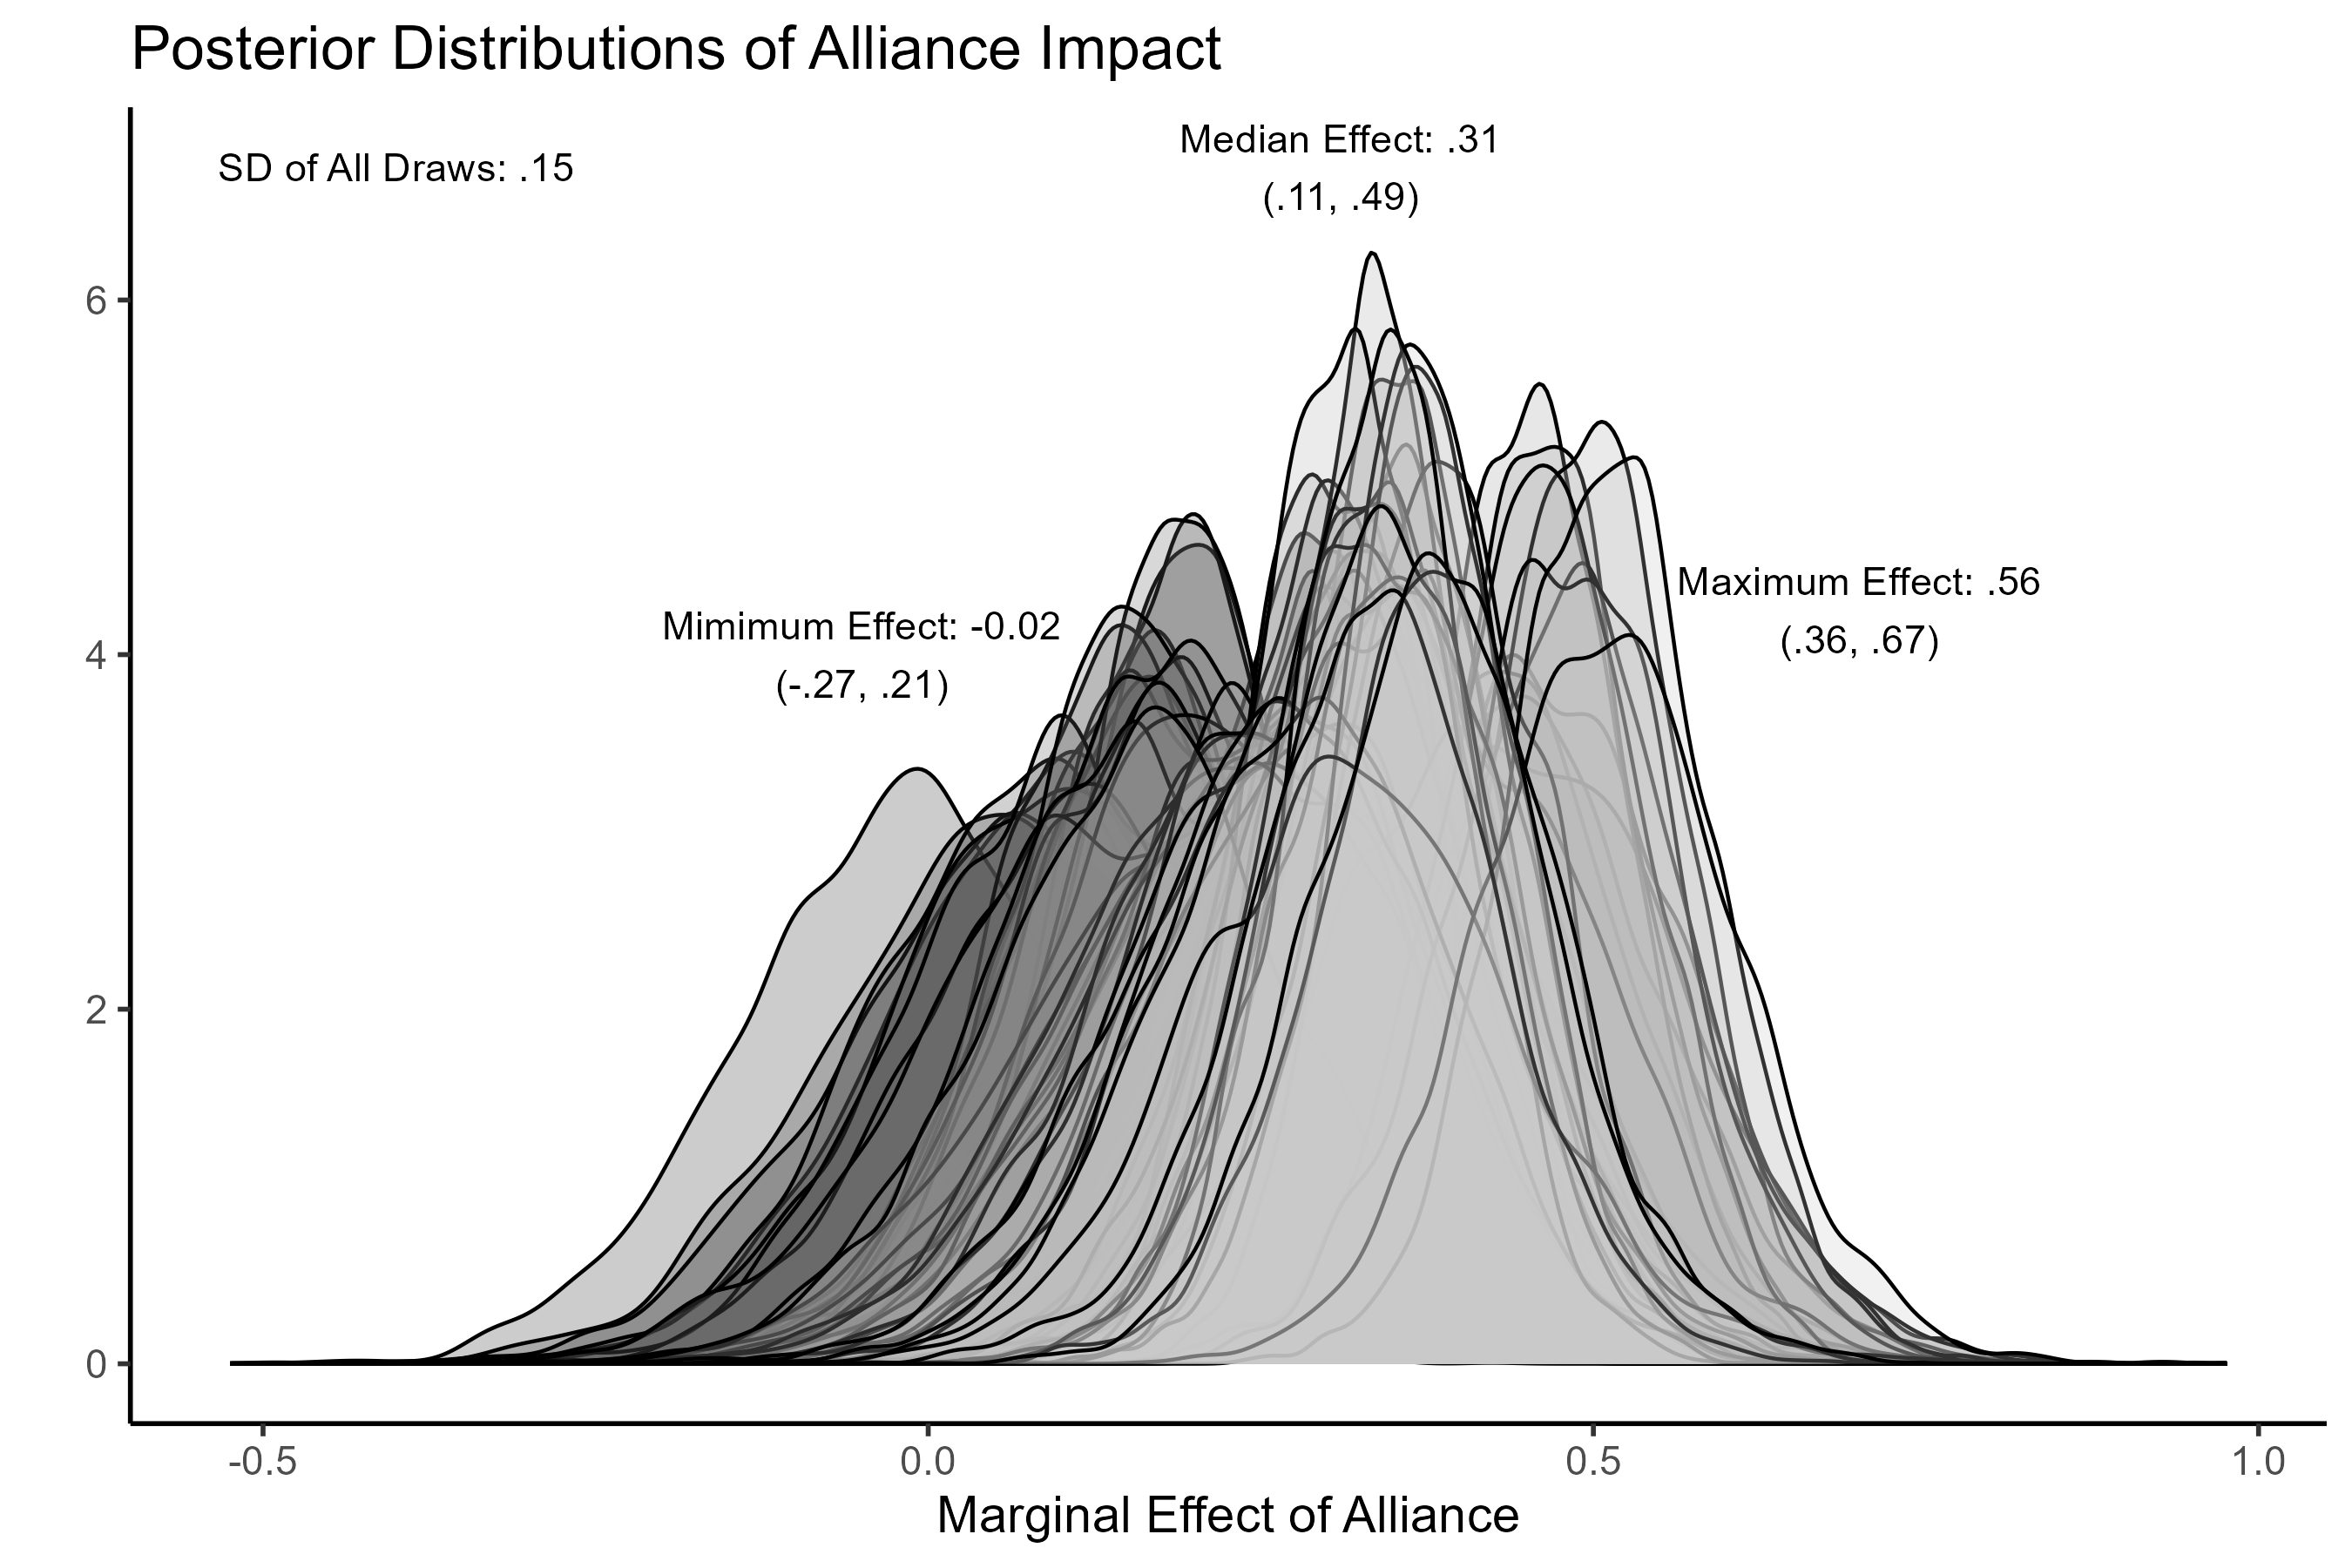
\includegraphics[width=0.95\textwidth]{../figures/tw-treat-het-sum.png}
	\caption{Posterior distribution of all estimated impacts of alliances on support for using force. Text values give notable point estimates, and parentheses summarize the 95\% credible interval.}
	\label{fig:tw-treat-het-sum}
\end{figure}


As a result of random variation and the systematic modification of group level variables I summarize in \autoref{fig:tw-het-source}, how alliances impact support for using force varies widely. 
\autoref{fig:tw-treat-het-sum} provides an initial summary of that variation, and highlights several noteworthy estimates. 


First, \autoref{fig:tw-treat-het-sum} notes that the minimum estimated impact of an alliance on a demographic group is .05, while the maximum is .53. 
The maximum effect occurs among white men with high internationalism and low hawkishness.
The minimum effect applies to non-white women with low internationalism and high hawkishness. 
There is no overlap in the posteriors of these estimates. 
The median group treatment effect estimate is .31, and this group of respondents is non-white men with middling internationalism and hawkishness. 
Alliances never clearly decrease support for intervention, but how much they increase support varies widely. 


\autoref{fig:tw-treat-het-sum} also presents the variation in how alliances impact demographic groups 
The standard deviation of all posterior draws is .13. 
Roughly 5\% of variation in the alliance effect is not explained by systematic regression components in \autoref{fig:tw-het-source}.\footnote{This is $\sigma_\theta$ above.}



\autoref{fig:tw-treat-het} provides an alternative presentation of the impact of alliances on support for using force that bridges \autoref{fig:tw-het-source} and \autoref{fig:tw-treat-het-sum}. 
As \autoref{fig:tw-het-source} and \autoref{fig:tw-treat-het-sum} suggest, alliances increase support for foreign intervention most among white men, especially those with low hawkishness and high internationalism.
By contrast, alliances have little impact on support for war among non-white females who are also skeptical of international engagement.
Individuals with more ambivalent foreign policy views respond more typically to TW's alliance treatment. 


\begin{figure}[htpb]
	\centering
		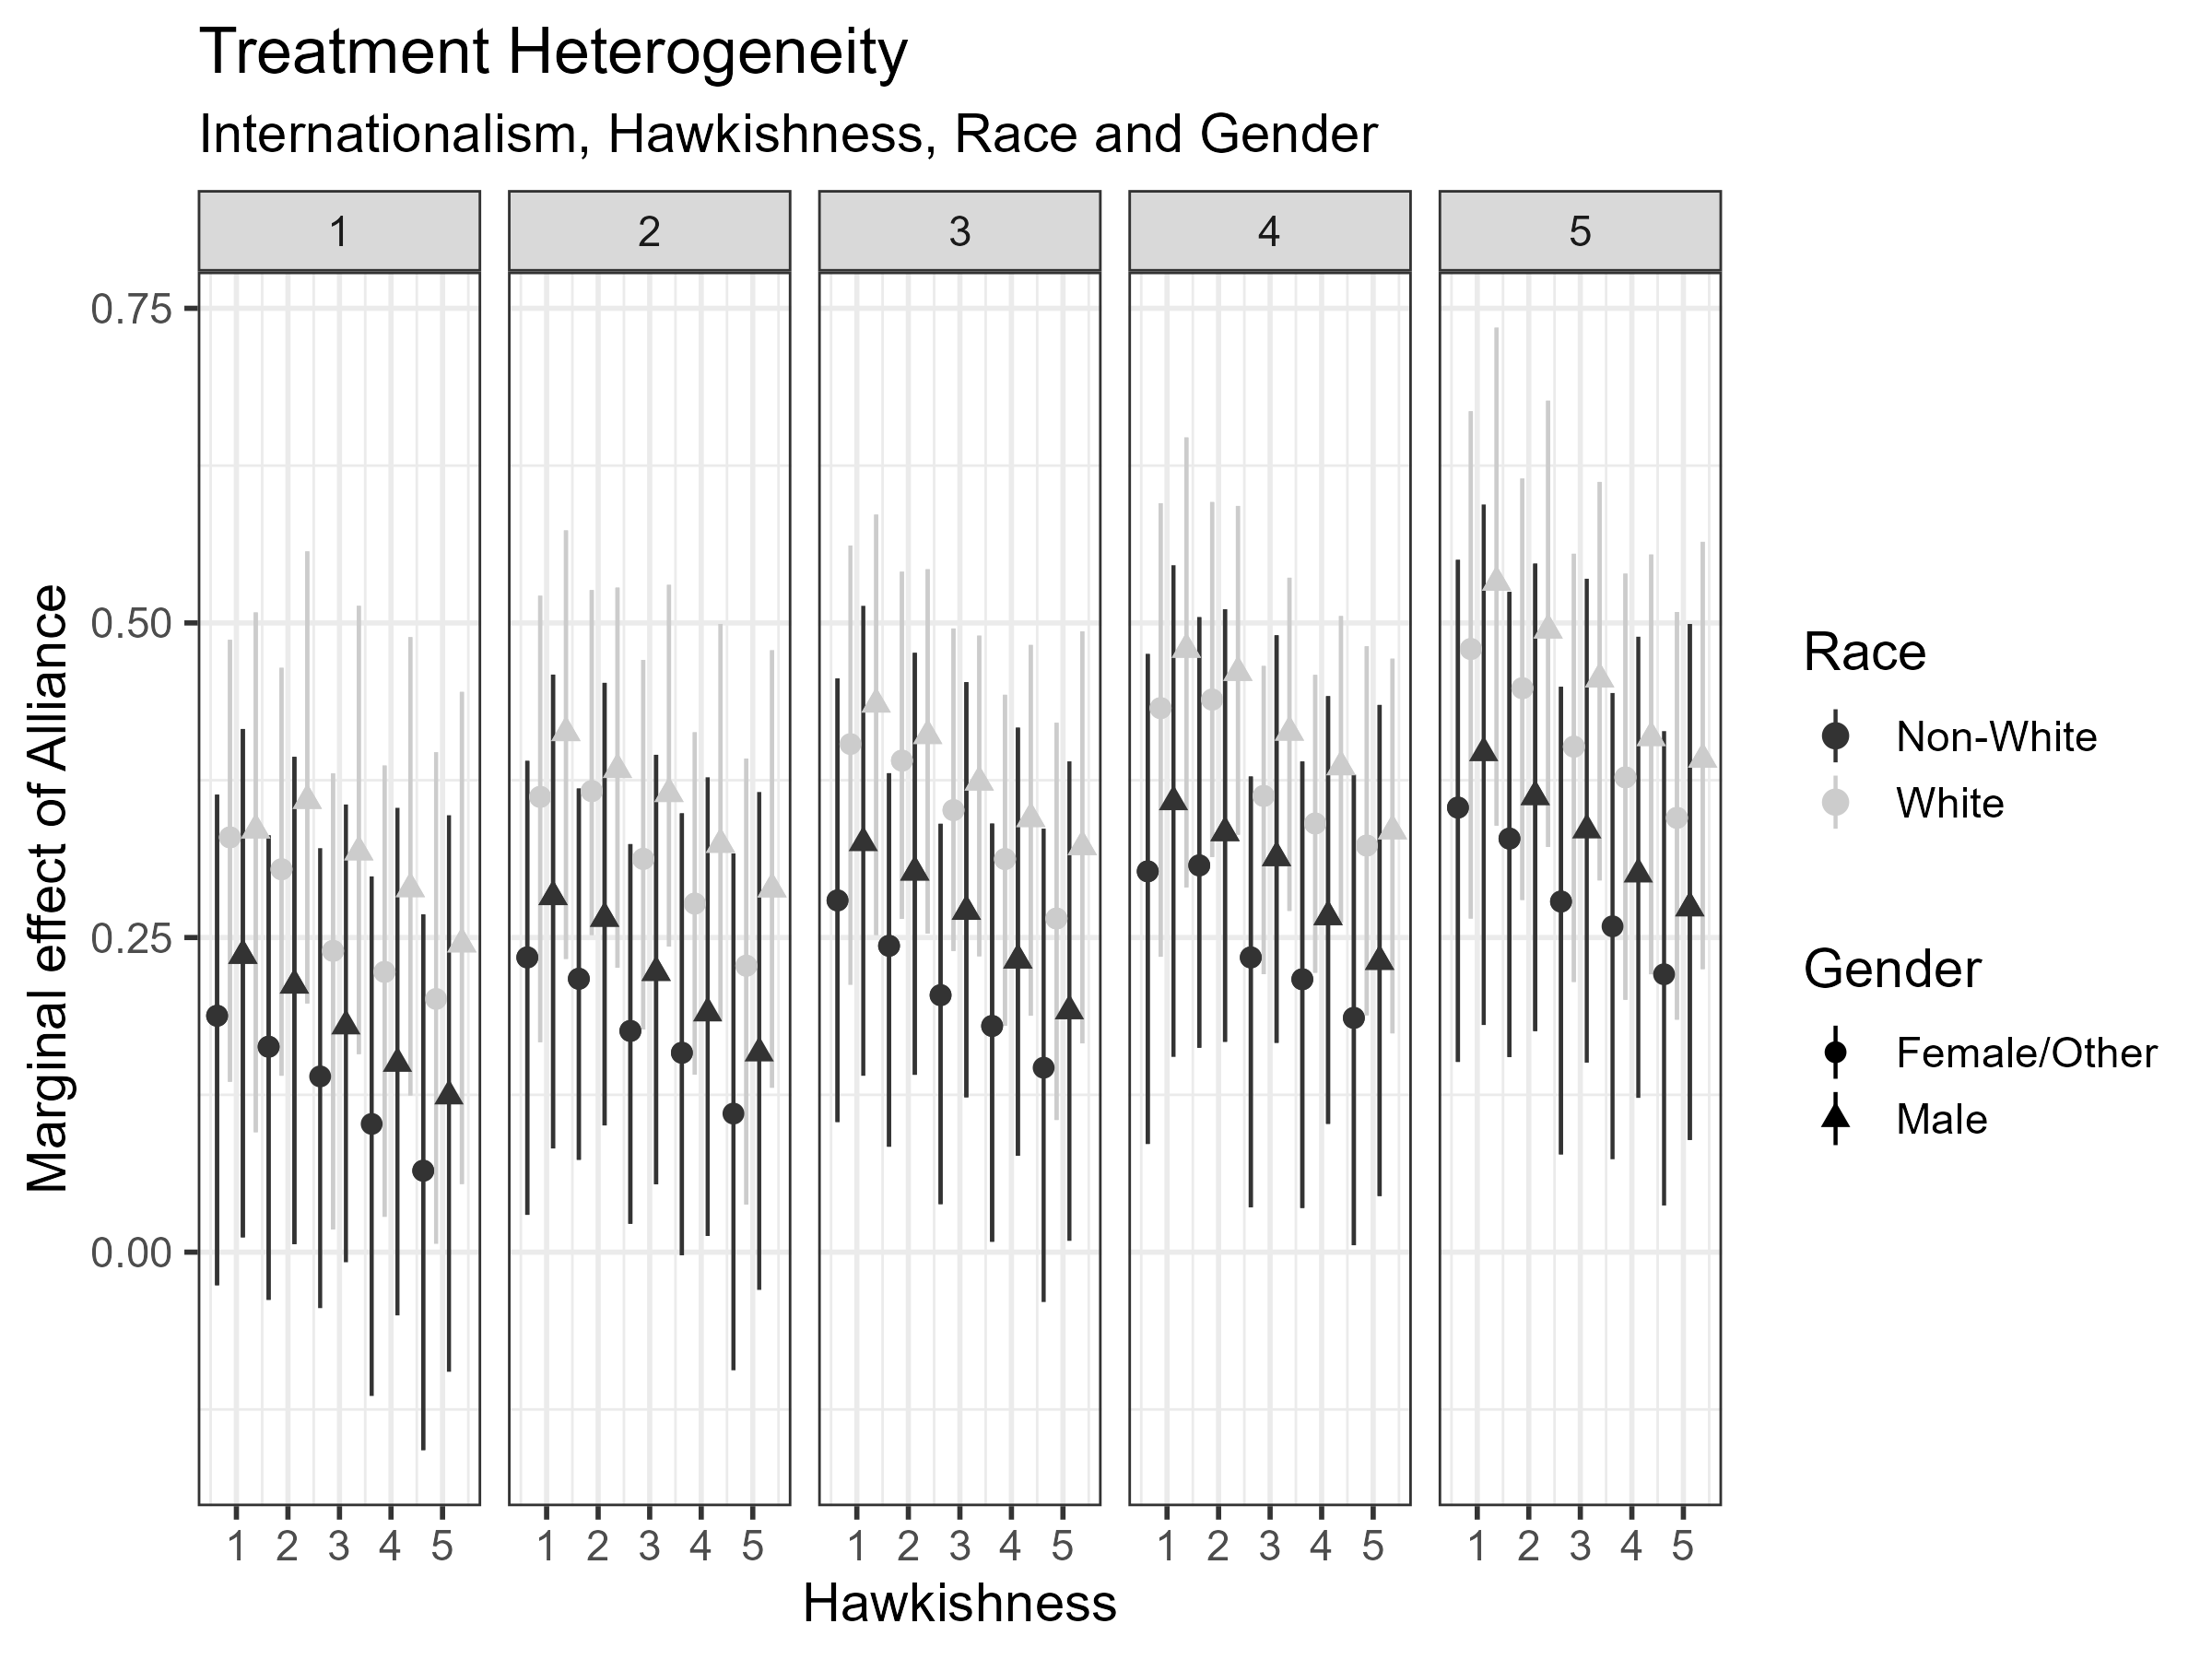
\includegraphics[width=0.95\textwidth]{../figures/tw-treat-het.png}
	\caption{Estimates of the impact of military alliances on support for using force within demographic groups. Column facets are values of internationalism, and row facets are levels of hawkishness. X-axis divided by gender and colors demarcate gender. Points mark the posterior median and bars summarize the 95\% credible interval.}
	\label{fig:tw-treat-het}
\end{figure}


All these estimates suggest that internationalism matters more than than hawkishness for understanding who is willing to fight for U.S. allies. 
Alliances may impact hawks less because these individuals support intervention regardless. 
Military alliances matter most to backers of international engagement who are otherwise less inclined to use force. 


% variation
These results show some of the strengths and weaknesses of the hierarchical approach to heterogeneous effects.\footnote{In the appendix, I analyze \citet{BushPrather2020}.}
A simple model based on demographic groups provides precise insights about who heeds alliances in supporting using force abroad. 
At the same time, because some demographic groups are small, the within-group effect estimates have substantial uncertainty and powerful comparisons between most groups is challenging. 
Fewer groups would have more data and less uncertainty but perhaps obscure variation across key demographic characteristics. 


\section{Conclusion}


This note explained how and when to use hierarchical models to estimate heterogeneous effects. 
Bayesian modeling can apply to a wide range of outcomes, data structures, and theories. 
It also details what drives variation in an effect and how much an effect varies. 
Explicitly modeling how different groups respond to an independent variable can help test arguments and inform policy.  


Hierarchical modeling provides an intermediate approach between interactions or subgroup analyses and machine learning algorithms. 
For interactions with one or two variables, relying on simple interaction tools is best. 
Similarly, machine learning is best for discovery of complex heterogeneity.
When there are two or more modifiers and many groups of theoretical interest, hierarchical modeling allows theoretically informed and interpretable estimation of effect variation. 

As a result, hierarchical modeling complements existing tools and should not replace them. 
Researchers can use hierarchical models to check and inform other techniques, for instance by seeing if a key interaction holds when there are multiple modifiers, or comparing multiple modifiers that past theories have identified. 
Using hierarchical modeling can thus help scholars and policymakers better understand heterogeneous effects.


\section*{Acknowledgements}

Thanks to Taylor Kinsley Chewning, Andrew Gelman and Carlisle Rainey for helpful comments.

\singlespace
\bibliography{../../MasterBibliography} 


%\documentclass[12pt]{article}

\usepackage{fullpage}
\usepackage{graphicx, rotating, booktabs} 
\usepackage{times}
\usepackage{fbb} 
\usepackage{natbib} 
\usepackage{indentfirst} 
\usepackage{setspace}
\usepackage{grffile} 
\usepackage{hyperref}
\usepackage{adjustbox}
\usepackage{multirow} 
\usepackage{amsmath}
\usepackage[labelfont={bf},textfont=it,labelsep=period]{caption}
\setcitestyle{aysep{}}
\usepackage{sectsty}
% for the big table
\usepackage{afterpage}
\usepackage{array}
\usepackage{lscape}
\usepackage{longtable}
\usepackage{float}
\sectionfont{\Large}
\subsectionfont{\noindent\large\textit}
\subsubsectionfont{\normalsize}


\singlespace
\title{\textbf{Appendix: Using Hierarchical Models to Estimate Heterogeneous Effects}}

\date{}
\bibliographystyle{apsr}

\begin{document}


\maketitle 

\singlespace 

\tableofcontents



\section{Tomz and Weeks Reanalysis}

This summarizes a heterogeneous treatments model of \citep{TomzWeeks2021} and details the underlying \textsf{R} code. 

\subsection{Heterogeneous Treatments} 

Here, I examine how the impact of alliances varies with other factors in the experiment, especially costs, stakes, region and partner democracy.
The heterogeneous treatment model corroborates TW's conclusion that alliances exert the greatest impact in instances when public opinion is otherwise skeptical of intervention.

\autoref{fig:tw-het-treat} supports TW's findings that alliances exert the most influence in situations where the public is otherwise unlikely to intervene. 
This figure shows the impact of alliances in unique combinations of all other experimental treatments. 
For a hypothetical democracy in Eastern Europe where intervention has high stakes, alliances exert minimal impact on public attitudes. 
In low-stakes and high cost interventions to support African, Asian or Latin American dictators, alliances increase support for intervention by 50\%. 
Beyond these systematic differences, random variation that is not attributed to the other treatments is roughly 6\%. 


\begin{figure}[htpb]
	\centering
		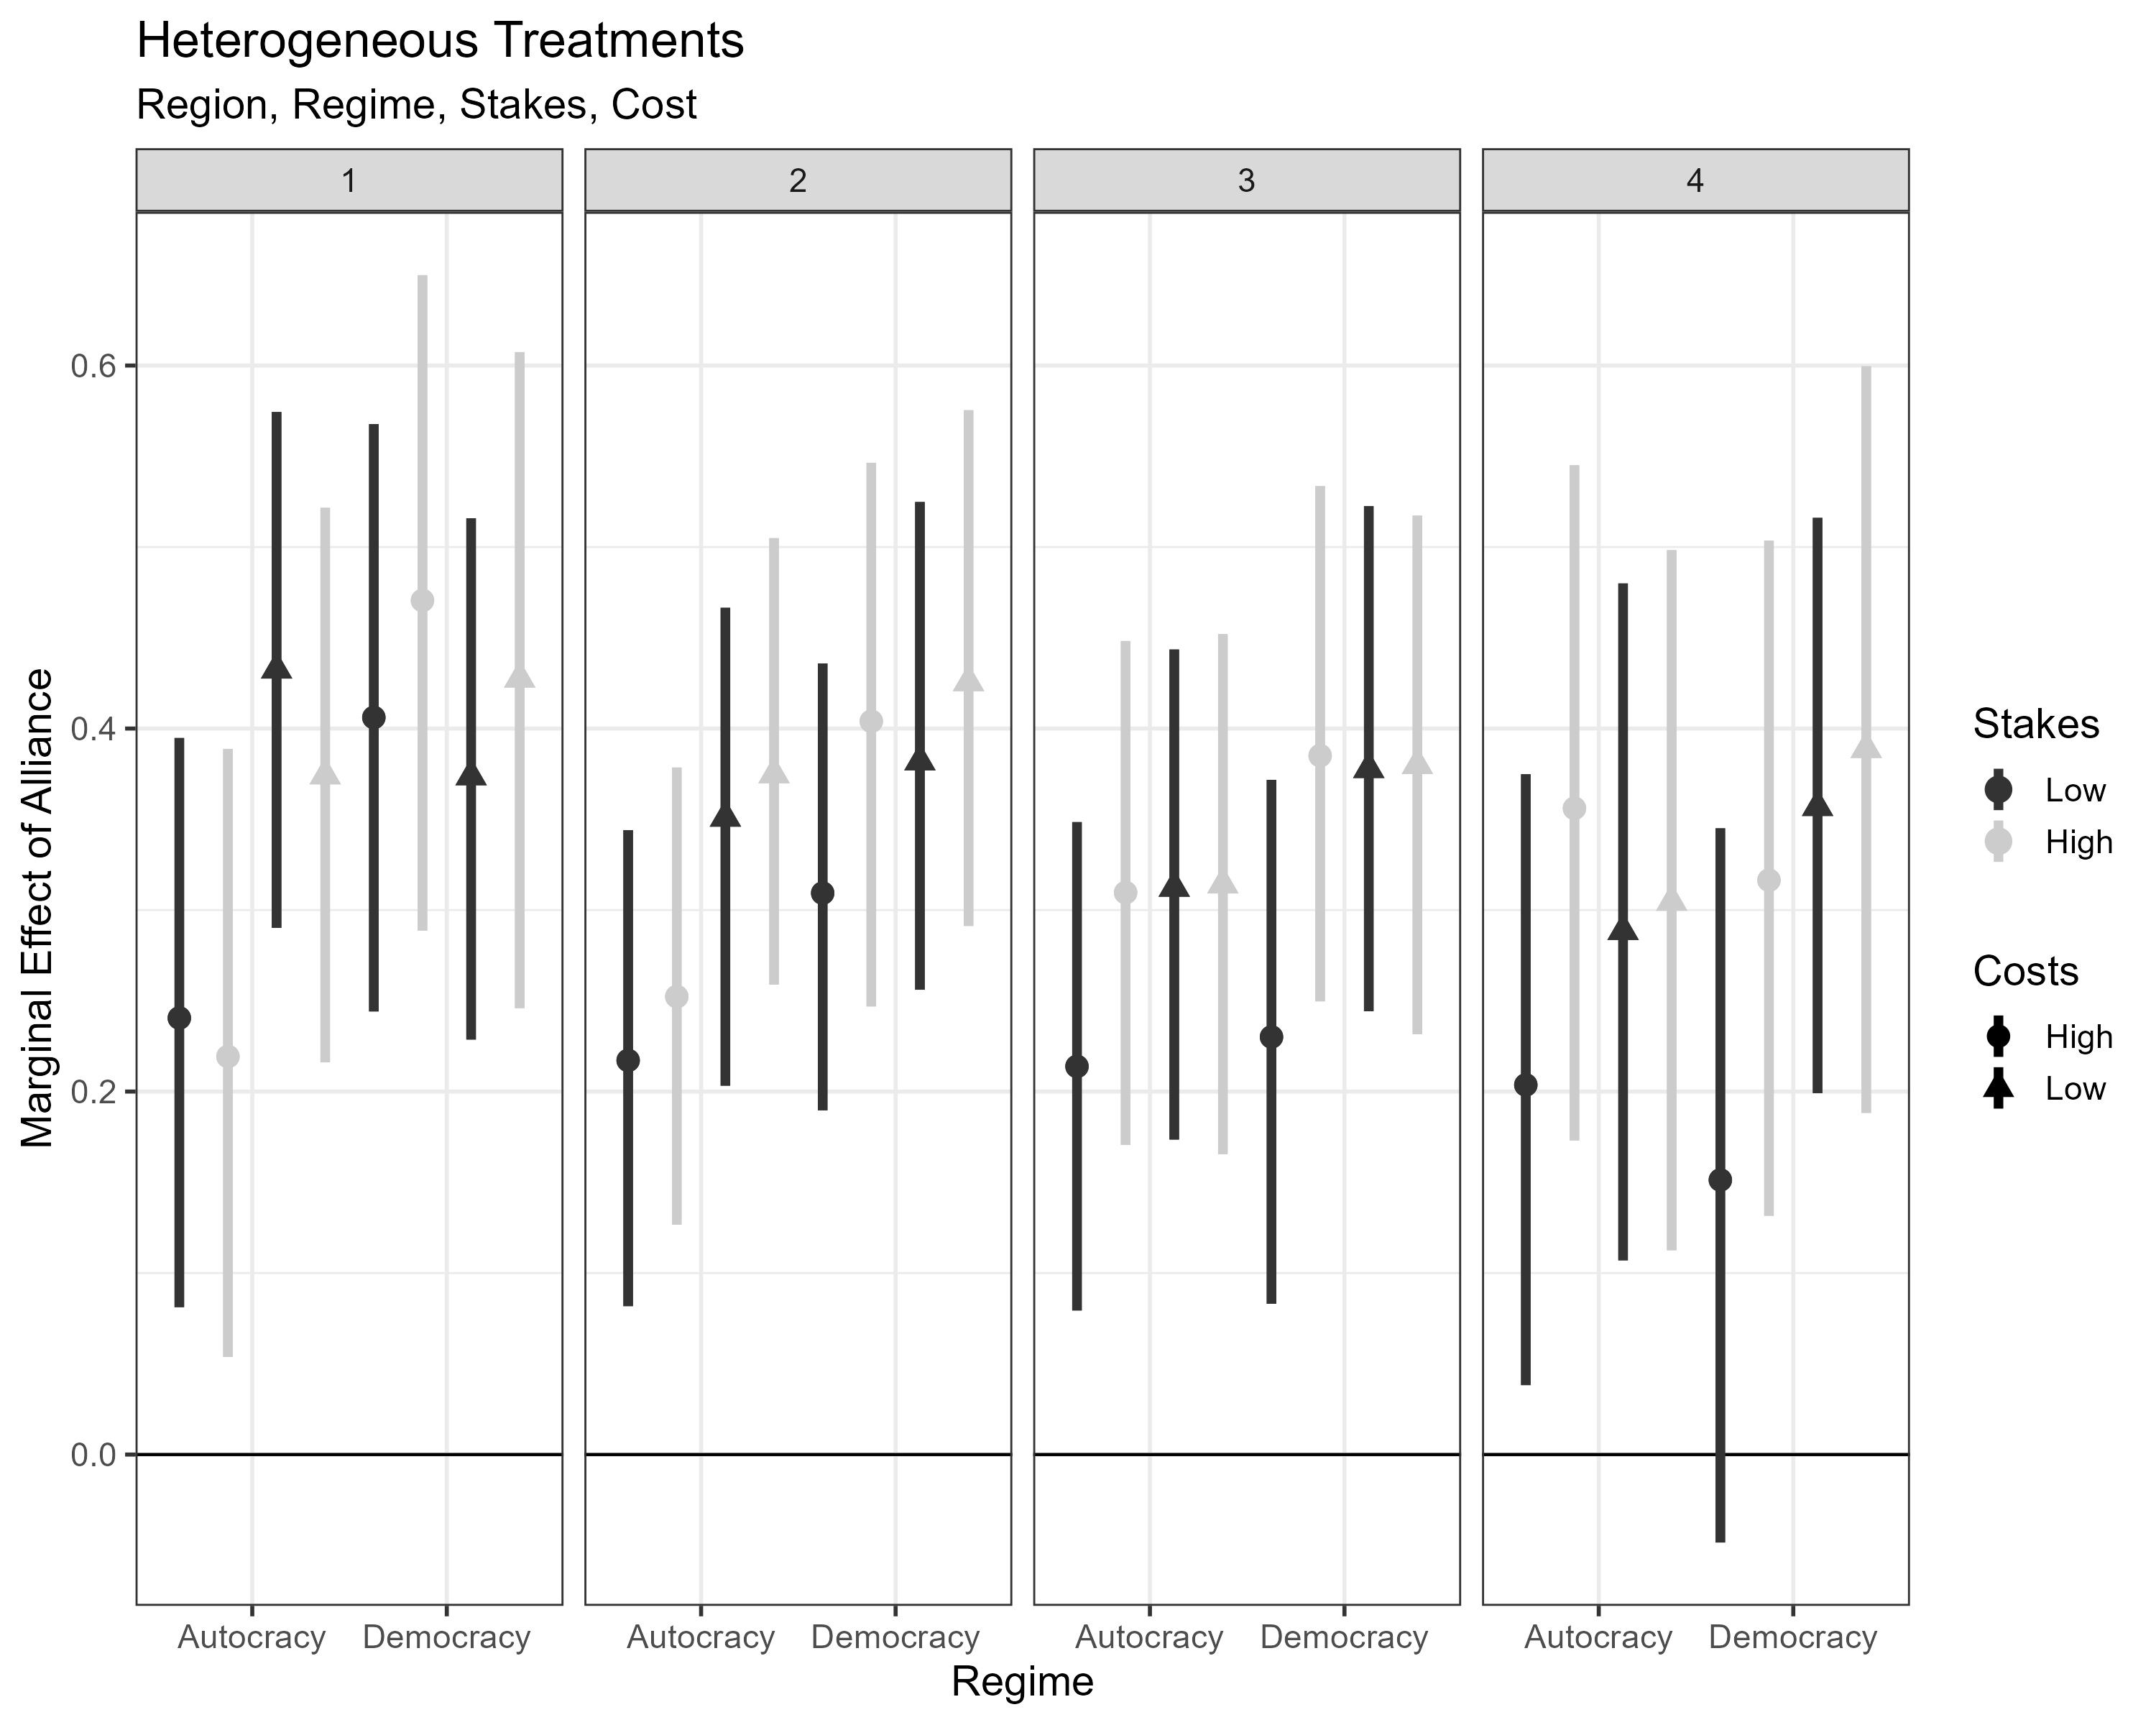
\includegraphics[width=0.95\textwidth]{tw-het-treat.png}
	\caption{Estimated impact of military alliances on public support for war across hypothetical region, costs, stakes and partner regime. Colors distinguish stakes, point shapes mark different costs, and estimates are grouped by regime type. Point estimates give the posterior median and error bars summarize the 95\% credible interval.}
	\label{fig:tw-het-treat}
\end{figure}


\subsection{R Code: Tomz and Weeks Reanalysis}

First, the following model formula expresses a heterogeneous treatments model where the impact of alliances varies with the regime under attack, the stakes, the costs, and the region. 
The \verb+treat.group+ indicator marks unique combinations of the regime, stakes, costs and region variables. 
It can also be written as \verb+regime:stakes:costs:region.txt+. 
I also control for gender, race, and three foreign policy dispositions. 

\begin{verbatim}
bf(force ~ 1 + white + male + hawk + intl + natl.sup + 
             alliance*(regime + stakes + costs + region.txt) + 
             (1 + alliance | treat.group) 
\end{verbatim}


The second formula expresses a treatment heterogeneity model where the impact of alliances varies with gender, race, and three foreign policy dispositions. 
The \verb+het.group+ indicator marks unique combinations of the demographic modifiers.
It can also be written as \verb+white:male:intl:hawk+. 
In this model, the other experimental conditions are controls. 

\begin{verbatim}
bf(force ~ 1 + regime + stakes + costs + region.txt +
             alliance*(white + male + intl + hawk) +
             (1 + alliance | het.group) 
\end{verbatim}



\section{Bush and Prather Reanalysis}


In the following, I again demonstrate how the model works by reanalyzing a study by \citet{BushPrather2020} (BP hereafter). 
This study examines how foreign meddling in elections impacts support for economic engagement with the meddler. 
One of their experiments examines how Russian or German engagement in the 2016 US election impacts mass support for trade and investment with those countries.
I use a heterogeneous effects model to check their results and further explore their findings. 


% describe design
BP employ a 2x2x2 factorial experiment.
This design randomizes whether a foreign country is interfering in the 2016 election, the country and their attitude towards Trump and whether the potential economic ties entail greater trade or investment in the United States.
In one treatment, Russia expresses support for Trump and in the other, Germany expresses opposition to Trump. 


BP hypothesize that individuals will prefer economic engagement with states that support their candidate. 
They thus examine how the impact of side-taking varies with the direction of the endorsement, individual political preferences, and the economic issue. 
To do this, they use four tables and figures, and rely on eight t-tests of differences in means between groups of roughly 25 respondents. 


The heterogeneous effects model encapsulates the argument and all tests by estimating the impact of side-taking on economic engagement as a function of which country is involved, a dummy indicator of intention to vote for Clinton, and their interaction. 
The interaction captures the hypothesis that Clinton voters will support engagement with Germany because Germany opposed Trump, and should be positive. 
I also add an indicator of whether the experiment deals with trade or investment. 
The heterogeneous effects equation also includes indicators of female gender and political engagement. 
The political engagement measure is a sum of political knowledge and interest. 


The outcome variable is a scale from one to four that measures support for greater economic engagement with the potential partner. 
To approximate BP's analyses, I use a normal outcome likelihood. 
Because this experimental randomization produced a roughly balanced sample, I do not include any control variables in the outcome equation. 


\begin{figure}[htpb]
	\centering
		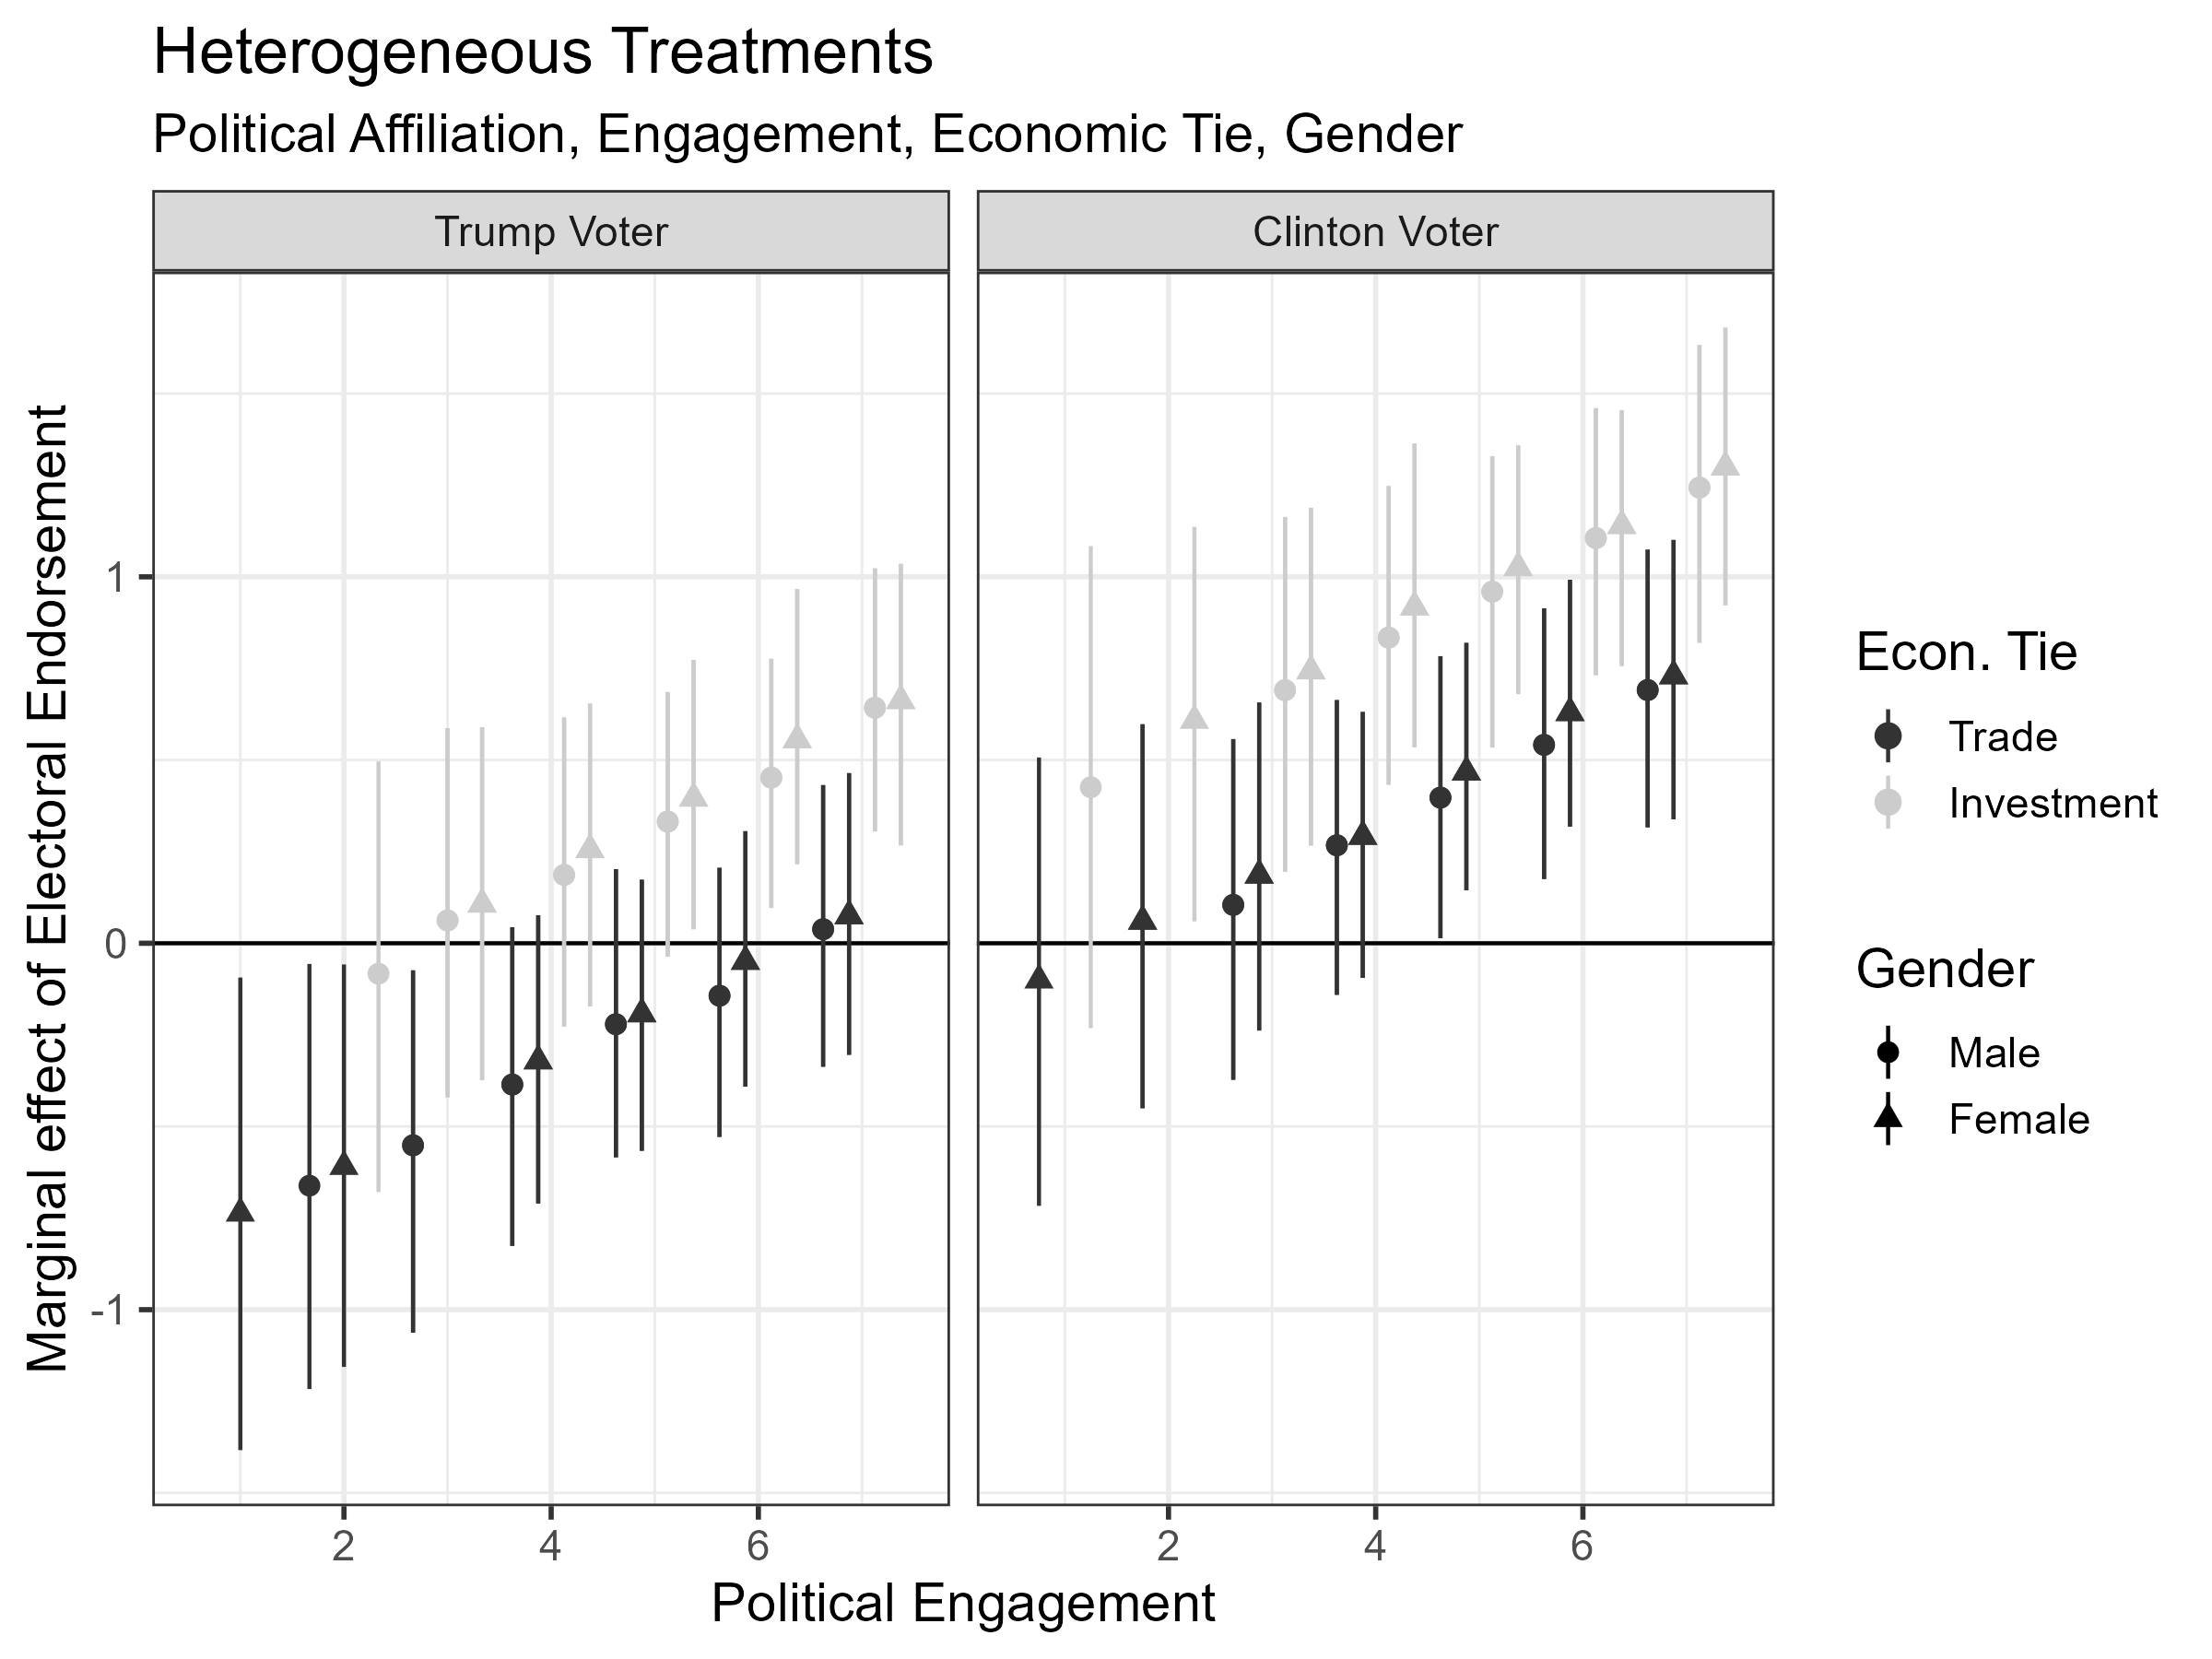
\includegraphics[width=0.95\textwidth]{bp-het-est.png}
	\caption{Heterogeneous effects of German side-taking in US elections on support for economic engagement with Germany. Each estimate reflects a treated group with a unique combination of other treatments and demographic characteristics.}
	\label{fig:bp-het-est}
\end{figure}


These estimates corroborate BP's findings, and also suggest that side-taking exerts the greatest influence on individuals who are highly engaged in politics. 
Clinton voters are more likely to support economic engagement with Germany when Germany has opposed Donald Trump. 
Conversely, some Trump voters oppose greater trade with Germany after the same side-taking. 
The impact of side-taking is also stronger for foreign investment than trade. 
Individuals are more willing to support investment than trade.


Side-taking exerts the most influence on individuals who are highly engaged in politics. 
Engaged Clinton voters respond most to German side-taking against Trump. 
Among these respondents, side-taking increases support for economic engagement by .5 or more, which is a large effect on an outcome that runs from one to four. 


\singlespace
 
\bibliography{../../MasterBibliography} 


\end{document}

\end{document}

